\chapter{Implementation}
\label{Chapter4}
\lhead{Chapter 4. \emph{Implementation}} % Write in your own chapter title to set the page header

In order to evaluate our proposed energy-aware gossip broadcasting protocol, we implemented the protocol in a open-source software called Network Simulator 3 (ns-3). From system point of view, this whole implementation consists of 4 major parts. They are the ICMP extension, the adaptive fanout \pp ~\gp, the UDP server and client application, and the simulation control program. The ICMP extension is the necessary backbone gossip communication infrastructure developed to support adaptive fanout \gp ~in application layer. The adaptive fanout \gp ~is the protocol entity that we are interested in studying. It utilized underlining ICMP extension to communication among gossip nodes. It controls our proposed adaptive fanout gossip protocol's logic and behavior. The UDP server and UDP client are installed on source node and gossip nodes respectively. This provides a channel to collect simulation data. Lastly, the simulation control program is developed to handle simulation environment set up, start and stop simulation, and process and output collected data.


\section{Basic Push-pull Gossip Protocol Implementation} \label{ppi}
\subsection{ICMP Extension}
For the basic push-pull \gp implementation, we first started building those 3 types of packets (Data packet, Ack packet, and Request packet) by extending the existing Internet Control Message Protocol (ICMP). The most common use of ICMP is for error reporting~\cite{james}. An ICMP message contains two parts: 8-byte header and data section. The first 4 bytes of the header have a fixed format. However, the last 4 bytes vary and depend on the type or code of the ICMP packet~\cite{forouzan}. The first and second byte of the header is the type field and code field respectively. And the third and fourth byte are checksum field. The format of the header is shown in Table \ref{table:1}.

\begin{table}[h!]
	\centering
	\caption{ICMP Header Structure}
	\label{table:1}
	\begin{tabular}{|p{1 cm}|p{1 cm}|p{1 cm}|p{1 cm}|p{1 cm}|}
		\hline
		Octet & 0 & 1 & 2 & 3 \\
		\hline
		& Type & Code & 
		\multicolumn{2}{ |c| }{Checksum}  \\
		\hline
		Octet & 4 & 5 & 6 & 7 \\
		\hline
		& 
		\multicolumn{4}{|c|}{Rest of Header}  \\
		\hline
	\end{tabular}
\end{table} 

Table \ref{table:2} here presented some of the selected ICMP message types. 

\begin{table}[h]
	\centering
	\caption{ICMP Control Messages}
	\label{table:2}
	\begin{tabular}{|p{1.5cm}|p{0.8 cm}|p{6.5 cm}|}
		\hline
		Type & Code & Description \\                                                           
		\hline
		0  & 0   & Echo reply   \\ \hline
		8  &  0 & Echo request \\ 
		\hline
		9 & 0 & Router Advertisement \\
		\hline
		10	& 0	&	Router discovery/selection/solicitation \\
		\hline
		42 to 255    &   & Reserved    \\ 
		\hline
	\end{tabular}
\end{table}

Since type 42 to 255 are reserved for further development, we decided to extend ICMP by defining type 42, 43, and 44 to represent Ack packet, Request packet, and Data packet respectively. The detail is shown in Table \ref{table:3}.

\begin{table}[h]
	\centering
	\caption{Our Gossip Protocol Extension}
	\label{table:3}
	\begin{tabular}{|p{0.8cm}|p{0.8 cm}|p{4.0 cm}|}
		\hline
		Type & Code & Description \\                                                           
		\hline
		42  & 0   & Send Acknowledgment   \\ \hline
		43  &  0 & Send Request \\ 
		\hline
		44 & 0 & Send Data \\
		\hline
	\end{tabular}
\end{table}

Based on these new control message types extension, we could further develop our basic \pp  ~\gp ~in ns-3. ICMP is a layer 3 protocol, but the actual control logic of our \gp ~is developed in application layer. 

\subsection{Source Node Implementation}
In order to generate and collect simulation results, the system consists of a source node and $n$ gossip nodes. The source node is responsible for the following duties:

\begin{itemize}
	\item Generate new broadcast \msgs
	\item Store time stamps for each generated new \msgs
\end{itemize}

Every time when a new broadcast \msg ~is generated, it will send it to one of the gossip nodes via a special pair of wireless ad-hoc network thus kick start the broadcasting process. Except the first broadcast \msg, every other new broadcast \msg ~will only be generated and sent out when it received $n$ \emph{Acknowledgment packet} (different from the Ack packet) from all gossip nodes for the previous broadcast \msg. Because in the program, we make sure that each gossip node will only send this special \emph{Acknowledgment packet }once per broadcast \msg, it is a good indication that this broadcast \msg ~has been successfully broadcast. In order to support this feedback mechanism, we deployed an UDP server application so that every gossip node can connect to it and send its \emph{Acknowledgment packet}. It is worth noting that the actual implementation of a source node is a streamlined \gn ~\im ~with functions in the receiving end and the ability to send Ack packets and Request packets disabled. 

\subsection{Gossip Nodes Implementation}
For gossip nodes, as shown in Figure \ref{fig:pseudo}, there are two main processes running. The periodic request processes and periodic gossip processes. At the start of the simulation, these two processes will be initialized. Most of the functionalities for a gossip node belong to either receiving end or transmitting end. In receiving end, we developed functions to handle Ack packet, Request packet, and Data packet. In the transmitting end, we developed functions to send Ack packet, Request packet, and Data packet. Besides, we also deployed an UDP client application on these gossip nodes so that it can send time stamps of each broadcast \msg ~back. To make all these functionalities work, these functions actually call the corresponding functions in ICMP as we described earlier. For example, if a gossip node is trying to send a new broadcast \msg ~to another gossip node, it would first call the function \emph{sendPayload()} that is in application layer. Then \emph{sendPayload()} would have to call the function \emph{sendMessage()} in ICMP which is in network layer. On the receiving end, a node first would receive the new broadcast \msg ~in network layer. The \msg ~is handled by a function in ICMP called \emph{handleData()}. Then in turn, this function will call the corresponding function in the application layer. The whole process is illustrated in Figure \ref{fig:topDown}.

\begin{figure}
	\centering
	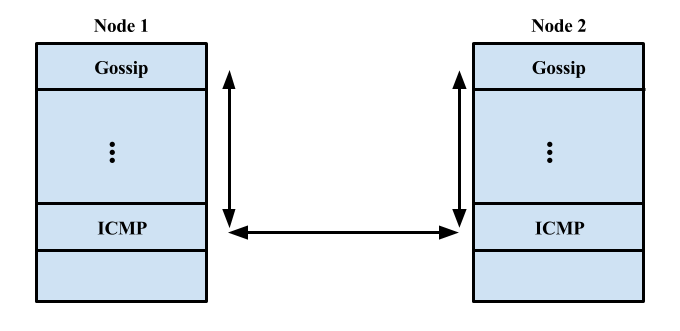
\includegraphics[width=5.5in]{topDown.png}
	\caption{An example of how two gossip nodes communicate}
	\label{fig:topDown}
\end{figure}

In summary, gossip nodes has the following responsibilities:
\begin{itemize}
	\item Gossip every new broadcast \msg
	\item Store every broadcast \msg without duplication
	\item Store the time stamps for each received new broadcast \msg
	\item Report each new broadcast \msg time stamps back to the source node
\end{itemize}

\section{Adaptive Fanout Extension Implementation}

To add our proposed adaptive fanout scheme into the existing \pp ~\gp, we first aggregated a basic energy source to each gossip node. Then we utilized WiFi radio energy model to simulate the energy consumption for each gossip node when transmitting or receiving a packet. The basic energy source increase or decrease its remaining energy linearly. The WiFi radio energy model has 4 states defined. They are TX, RX, IDLE, and SLEEP. The power consumption of each state in Watts are defined as follow:

\begin{itemize}
	\item $P_{tx}=1.14$
	\item $P_{rx}=0.94$
	\item $P_{idle}=0.82$
	\item $P_{sleep}=0.10$
\end{itemize}

In our implementation, we actually set $P_{idle}=0$ and $P_{sleep}=0$ because majority of the time when a node participated in broadcasting a \msg, it stays in the IDLE state. Therefore, it we don't disable $P_{idle}$ and $P_{sleep}$, the network lifetime will be largely determined by $P_{idle}$ which is undesirable. Once we have energy sources and Wifi radio energy model installed on the gossip nodes, we then can calculate the corresponding \emph{Fanout} for each node. One small detail worthing mentioning here is that the actual \emph{Fanout} $f_{actual}$ cannot exceed a node's degree (number of neighbors) $n_b$, thus $f_{actual} = min(f, n_b)$. Once we have the \emph{Fanout} information, the rest gossip process works as described in Section \ref{ppi}.

\section{Simulation Control Program}

As we stated earlier in this chapter, the simulation control program is here to properly set up simulation environment, initialize simulation objects, start and stop simulation, and collect, process, and export simulation data.

For the simulation environment set up, because we want to collect simulation data about network lifetime, the simulation stop time is set to be large enough so that the energy source will be depleted first. Any depleted energy source will automatically trigger the simulation to stop. Topology wise, we wanted it to be a close resemble to Wireless Sensor Network (WSN) or MANET. In other words, we wanted to avoid gossip nodes cluster in a small area. We achieve that goal by adopting a small maximum WiFi range for each gossip node and scale up nodes' placement area as number of nodes increases. Since an area with dimension of $100m \times 100m$ with $50m$ maximum WiFi range can achieve a desirable network density for 10 gossip nodes, we used this ratio to calculate the dimension of nodes placement area. If we denote the side of a square area by $s$, then the equation to calculate the size of the nodes placement area is as follows:

\[ s=\sqrt{1000\times n} \quad \mbox{where } n \mbox{ is number of gossip nodes}\]

Because of random gossip nodes placement and a fixed maximum WiFi range, a newly generated topology could contain isolated nodes that no other nodes can contact. In this case, we cannot achieve successful broadcasting no matter what we do. Another possible case is shown in Figure~\ref{fig:twoSepNet} where a network is divided into two separated subnets unconnected. In this case, none of the gossip nodes are isolated but we still cannot successfully broadcast a \msg. Therefore, we applied Depth First Search (DFS) algorithm to ensure that all nodes in the network are connected in some way. Based on each gossip node's neighbor list, DFS would try to traverse all gossip nodes starting from any gossip node. If the algorithm is able to visit all gossip nodes, we consider this newly generated topology suitable for our simulation. On the other hand, when the algorithm cannot traverse all gossip nodes successfully, this simulation instance will be terminated.

\begin{figure}
	\centering
	\includegraphics[width=4in]{twoSepNet.png}
	\caption{An example when two separate subnets formed}
	\label{fig:twoSepNet}
\end{figure}

As mentioned earlier, DFS algorithm need each \gn's neighbors list in order to properly perform. To obtain this information, after the random \gn placement, the program can access each node's coordinates. Assuming node 1 ($node_1$) has the coordinate of $(x_1, y_1)$ and node 2 ($node_2$) has the coordinate of $(x_2, y_2)$, the distance between $node_1$ and $node_2$ can be easily computed by the distance formula. Therefore, if we denote the distance between $node_1$ and $node_2$ is $d$, then $d = \sqrt{(x_1 - x_2)^2+(y_1 - y_2)^2}$. Now if we denote each \gn's WiFi range to be $R$, then $node_1$ and $node_2$ are neighbors when $d\leq R$. While $node_1$ and $node_2$ are not neighbors when $d > R$. We used this process to generate neighbors list for each \gn. In practice, the global access of each \gn's coordinate information is usually not easy to obtain. Thus, Hello packets are used to generate neighbors list for each \gn.

The work flow of our simulation control program is described below. 

\begin{itemize}
	\item Read in simulation environment parameters. 
	\item Create a source node and $n$ gossip nodes.
	\item The wireless ad-hoc network channel speed is set to be 1Mbps for all \gns.
	\item Create a special wireless ad-hoc network connection between a source node and a \gn and set its speed to be 11Mbps.
	\item Compute the side size of a square area for nodes placement.
	\item Randomly place all nodes in the square area
	\item Install basic energy source and \wf ~radio energy model on the \gns.
	\item Assign IP addresses to all nodes.
	\item Install adaptive fanout \gp and UDP client application ~on the \gns.
	\item Install gossip generator application and UDP server application on the \sn.
	\item Generate neighbors list for each \gn.
	\item Check topology connectivity using DFS algorithm.
	\item If the topology is disconnected somehow, terminate this simulation.
	\item If the topology is connected, start the simulation.
\end{itemize}

The link speed among \gns is set to be 1Mbps because it is sufficient to transmit a very small Data packet quickly. The link speed between the source node and one of the \gn ~is set to be 11Mbps because we want to make sure that source node does not become the bottleneck for the performance of our proposed \gp. Since all nodes including the source node are randomly placed in this area, we make sure that the \wf ~range of the \sn ~is large enough that it will always be able to reach any \gns. The \wf ~range of \gns ~is set to be 50m in order to control node's degree. 

As we stated earlier, the simulation will stop once any \gn's energy is depleted. From that point, the program will enter the data collection and process stage. At this stage, the program is trying to calculate the following data:

\begin{itemize}
	\item Message broadcast time (one output file per simulation)
	\item Average overhead per node per \msg ~(average within each simulation)
	\item Average energy consumption per node per \msg ~(average within each simulation)
	\item Network lifetime
\end{itemize}

For the \msg ~broadcast time, the program will access the vector stored in the \sn ~that represent the time stamps for each generated new broadcast \msg. Similarly, it will also access $n$ vectors from $n$ \gns. These vectors stored the received broadcast \msg ~time stamps of each \gn. Let's take a look at an example where we have one \sn ~and one \gn and the protocol successfully broadcast $m$ \msgs, if we denote the vector on the \sn ~side to be $T_s=<t_{s1}, t_{s2}, \ldots, t_{sm}>$ and the vector on the \gn ~side to be $T_g=<t_{g1}, t_{g2}, \ldots, t_{gm}>$, then the delay for these \msgs ~are $T_{delay}= T_g - T_s = <t_{g1}-t_{s1}, t_{g2}-t_{s2}, \ldots, t_{gm}-t_{sm}>$. For the scenario where $n$ \gns participated in the broadcasting process, because we are interested in \msg ~broadcast time, the program will first calculate the $T_{delay}$ for each \gn ($T_{delay_1},T_{delay_2},\ldots,T_{delay_n} $). Then it will loop through the first element in those vectors and store the maximum delay because by our definition for one broadcast \msg ~the time difference between the last \gn received the \msg ~and the time the \sn ~generate that \msg is the broadcast time for that \msg. And then the program will repeat that process until it reaches the $m_{th}$ broadcast \msg. However, we would like to point out that this process is only applied on a per simulation basis. To obtain the data that later our performance metrics need, further process need to be done.

For the overhead, we defined it as the total number of packets this protocol sent during the simulation. This includes Ack packet, Request packet, and Data packet. Our simulation control program first will access the \emph{packetSent} counter on each \gn. Then it will average over total number of broadcast \msgs ($m$ \msgs). Finally, it will take that number and average over number of \gns ~($n$ gossip nodes). Again, this process is done in a per simulation basis. Further data process is needed to yield our desired performance metrics data.

Similar to the process of calculating average overhead per node per \msg, in order to compute average energy consumption per node per \msg, the program would first collect consumed energy from the \gns, and then average over number of \gns ~($n$). And finally it will take that number and average over total number of broadcast \msgs ~($m$). 

The network lifetime is defined as the time duration which all \gns ~have energy to receive and transmit packets. Therefore, as we stated earlier, when any \gn's energy is depleted, That moment is consider the end time of our simulation. And the program simply output the simulation stop time to a file.
